

%*************************************************************************
% Chapter Quote
\begin{savequote}[50mm]
‘‘Equipped with his five senses, man explores the universe around him and 
calls the adventure Science’’
\qauthor{Edwin Hubble}
\end{savequote}
%*************************************************************************


\chapter{Introduction}
\label{cha:Introduction}

 
%*************************************************************************


‘‘What is our place in the cosmos?’’ This is one of the more simple and 
trans\-cendental question of the human beings, and powered by our innate 
curiosity has led to a current relatively understandable picture of our 
Universe. In fact, the astronomy can be only considered as a scientific 
rigorous discipline after the seventeenth century.


%*************************************************************************





%*************************************************************************
%Prehistory
\section{Prehistory}
\label{sec:Prehistory}


Almost in every scientific discipline a significant theoretical advance is 
accompanied of a technical improvement of its own instruments, it is for 
this reason that at the beginning of the seventeenth century Johannes Kepler 
could establish his three well-known empirical laws of the planetary 
movements based on the very precise data of astronomical bodies computed 
for Tycho Brahe. This event was very remarkable in the astronomy history 
due to was the first of many strikes against the well established 
anthropocentric notion of the cosmos. Although the Kepler laws constituted 
the most crucial test to the Nicolaus Copernicus heliocentric model, it was 
only until 1685 when Isaac Newton formulated the law of universal gravitation 
(from which can be derived all the Kepler laws) when the astronomers could 
have a enough powerful tools to begin a depth and serious discussion about 
the real nature of our universe on scales bigger than the solar system, and 
thus inaugurating the \textit{sciences of gravity} \cite{longair2008}.



After the establishment of the universal gravitation, the next significative 
theo\-retical achievement in this area came in the centuries eighteenth and 
nineteenth with the development of classical mechanics, as the Hamiltonian 
and Lagrangian formalism, and powerful numerical tools. All this achievements 
impulse the study of key topics as the many body problem, allowing a depth 
understanding of the dynamic of complex gravitational system, as planetary
system, star clusters, etc. 



Parallel to previous theoretical advances, in the observational side was 
beginning to arise the idea of \textit{island universe}, from which will 
evolve the concept of galaxy. This was powered by the development of the 
telescope, allowing besides to understand that the galaxy is only a large 
collection of stars like our sun. It was very remarkable the pioneer work of 
William Herschel, who tried to make a map of our galaxy determining distances 
with the assumption that stars have the same intrinsic luminosity and the 
inverse square law for the intensity decay (see figure \ref{fig:HerschelModel}). 
Although his results were very imprecise due to the incorrect assumption on 
which were based, the importance of his work lies in the recognition of a 
structure (disk-like) for our galaxy. 


%.........................................................................
%Herschel Model of Our Galaxy
\begin{figure}[htbp]
	\centering
	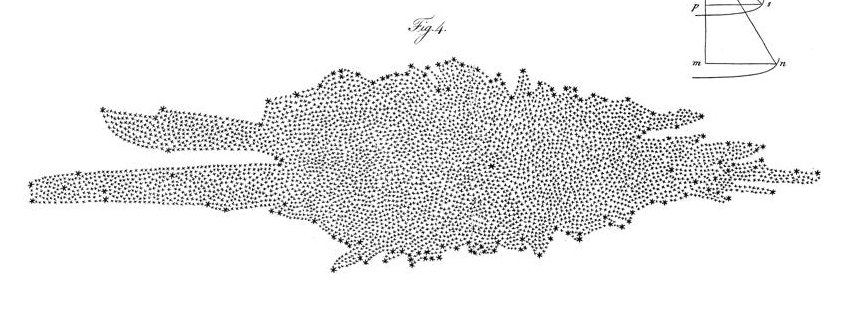
\includegraphics[width=1.0\textwidth]{./figures/1_introduction/Herschel_Model.png}
	
	\caption{\small{William Herschel's model of our galaxy based upon star 
	counts and the equal luminosity assumption.\cite{Herschel1785}}}
	
	\label{fig:HerschelModel}
\end{figure}
%.........................................................................


Another important observational question that was emerging in that epoch 
is the existence of \textit{island universes} like ours. It was already 
well-known the existence of extended objects that do not fit to definition 
of stars or planets, as nebulae, planetary disks and galaxies. Even William
Herschel and his son John Herschel contributed with the realization of an
large (for the epoch) catalogue of extended bodies known as 
\textit{Catalogue of Nebulae and Clusters of Stars} and an expanded version
finished by John Dreyer in 1888, \textit{New General Catalogue of 
Nebulae and Clusters of Stars}, which together with \textit{Index Catalogues}
of 1895 and 1908 constitute a large collections of bodies widely used in 
current astronomy, referred with the abbreviations \textit{NGC} and 
\textit{IC} respectively \cite{longair2008}. Despite of this observational
advances, the real nature of this objects was a complete mystery, especially 
if they lie within our own galaxy or are completely independent systems. 



This question remained until twentieth century and together with the real 
size of the universe were the two big issues treated in the well-known 
\textit{Great Debate}, also called the \textit{Shapley-Curtis Debate}, an
important event in the history of astronomy where the astronomers Harlow 
Shapley and Herber Curtis gave respectively different arguments in favour 
of and against the belonging of these objects to our galaxy and the Milky 
Way as our whole universe. Despite of this, their arguments were not very
conclusive and the solution to these issues had to wait until 1924 when 
Edwin Hubble measured the distance to Andromeda Galaxy (M31 or NGC 224)
and demonstrated unquestionably the real extragalactic nature of this 
object, and in the following years for other ones. This achievement together
to the observational verification of expanding universe (also due to Hubble)
were the beginning of modern observational cosmology.



It also happened in the twentieth century a key event for the modern 
sciences of gravity, Albert Einstein formulated his theory of General 
Relativity, changing completely the previous conception of space and time 
and laying the foundation of current cosmology picture.


%*************************************************************************




%*************************************************************************
%The current cosmology picture
\section{The Current Cosmology Picture}
\label{sec:TheCurrentCosmologyPicture}


The conceptions of space and time were misunderstanding before 1900 century
and their connection with the gravitational interaction was completely 
neglected, both key issues for the adequate understanding of our universe,
it is for these reason that the formulation of the General Relativity opened
the door to a complete set of theoretical tools


%*************************************************************************




%*************************************************************************
%Cosmological observations
\section{Cosmological Observations}
\label{sec:CosmologicalObservations}
	
%*************************************************************************




%*************************************************************************
%Numerical simulations
\section{Numerical Simulations}
\label{sec:NumericalSimulations}


%*************************************************************************